\documentclass[11pt,a4paper]{article}
\usepackage[utf8]{inputenc}
\usepackage[T1]{fontenc}
\usepackage{amsmath}
\usepackage{amsfonts}
\usepackage{amssymb}
\usepackage{graphicx}
\usepackage{booktabs}
\usepackage{array}
\usepackage{float}
\usepackage{geometry}
\usepackage{setspace}
\usepackage{caption}
\usepackage{subcaption}

\geometry{margin=1in}
\onehalfspacing

\title{Sample}
\date{\today}

\begin{document}

\maketitle

\section{Figures}

\begin{figure}[H]
    \label{fig:news_trends}
    \caption{Number of firms}

    \begin{center}
    Panel A. Average Number of News Articles per Month
    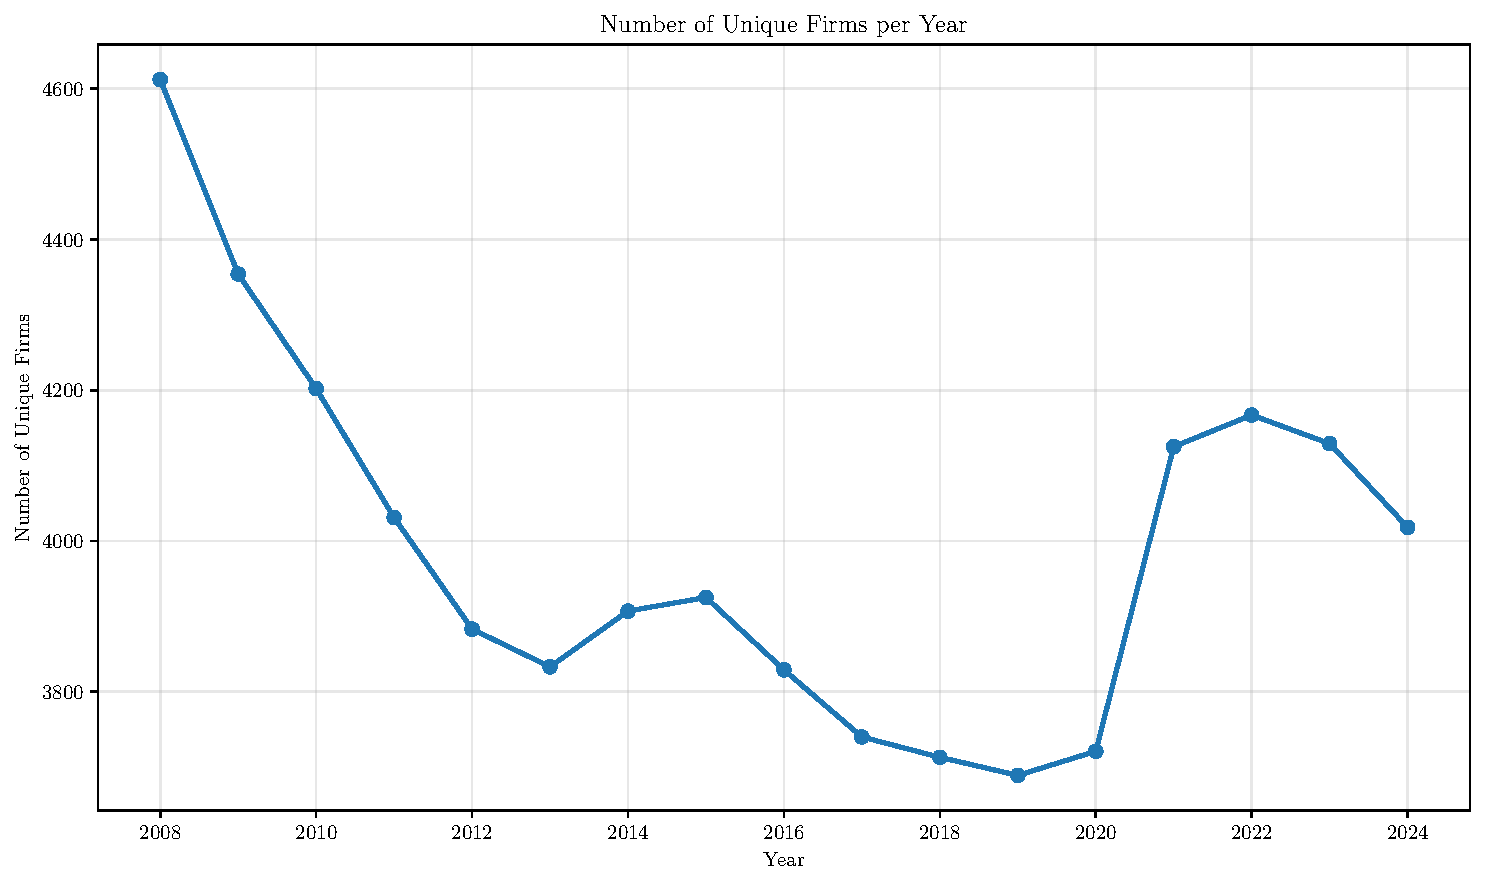
\includegraphics[width=0.6\textwidth]{../results_figures/n_stocks_per_year.pdf}
    \end{center}

\end{figure}

\begin{figure}[H]
    \label{fig:fomc_premium}
    \caption{The FOMC announcement premium}

    \begin{center}
    Cumulative market excess return, scheduled FOMC announcement days vs.\ all other days
    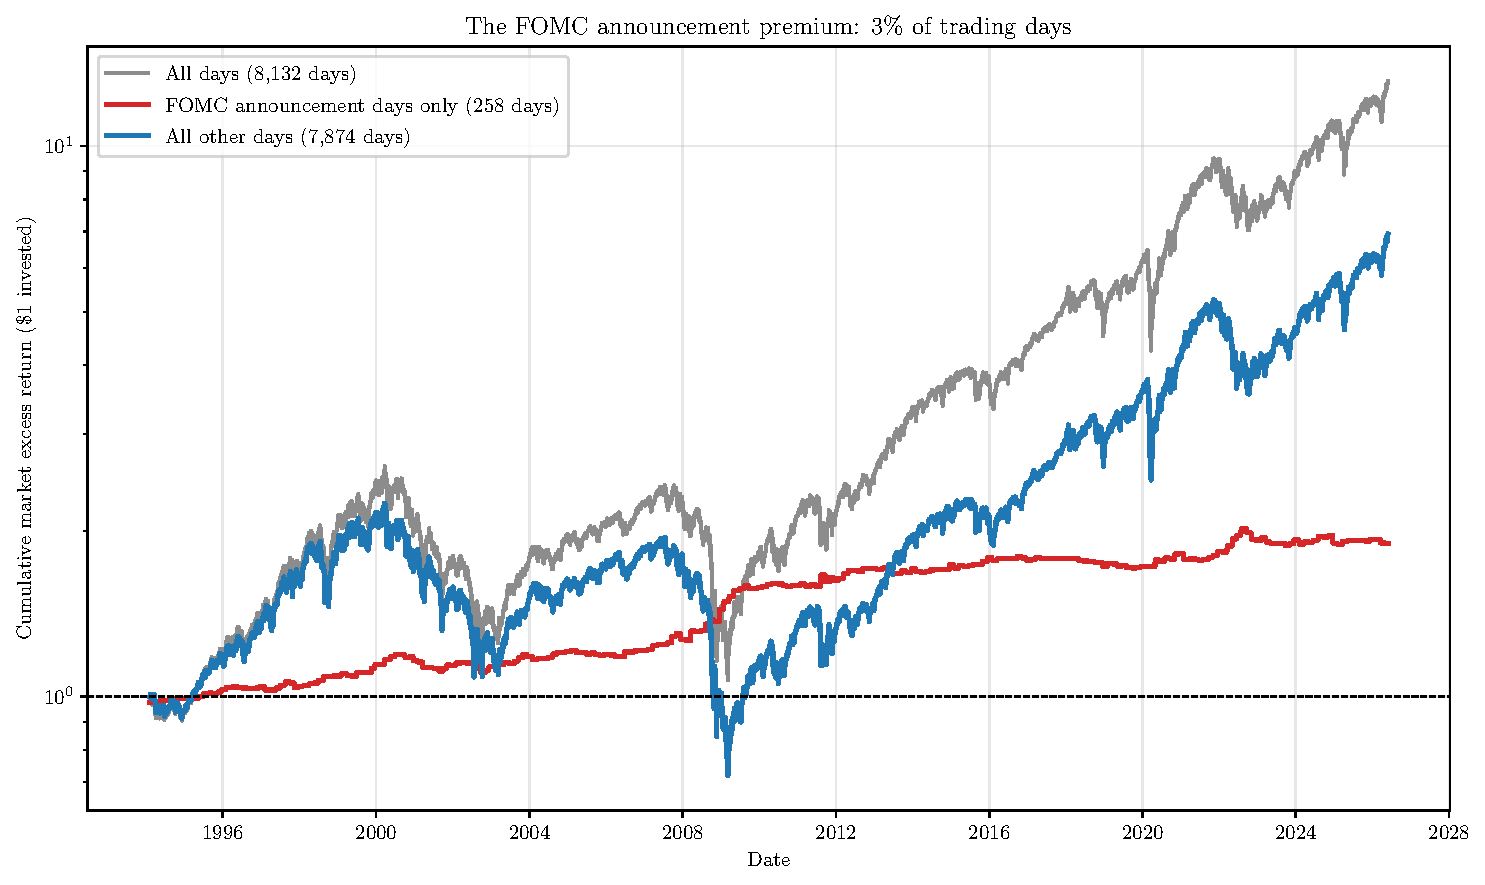
\includegraphics[width=0.8\textwidth]{../results_figures/fomc_premium.pdf}
    \end{center}

\end{figure}

\newpage

\section{Tables}

\begin{table}[H]
\label{tab}
\resizebox{1\textwidth}{!}{%
\input{../results_tables/ea_regression.tex}
}
\end{table}

\begin{table}[H]
\caption{The FOMC announcement premium}
\label{tab:fomc_premium}
\centering
\footnotesize
\begin{tabular}{rccccccc}
\hline\hline
{} & \multicolumn{7}{c}{Dependent variable} \\
{} & \multicolumn{5}{c}{$Ret^M-R_f$ (\%)} & $\Delta VIX$ & $VIX$\\
{} & Full & Leads/lags & 1994--2010 & 2011-- & Ex 2008--09 & Full & Full \\
{} & (1) & (2) & (3) & (4) & (5) & (6) & (7)\\
          \cmidrule(lr){2-6}  \cmidrule(lr){7-7}  \cmidrule(lr){8-8}
$1_{FOMC,-1}$ &  & 0.073 &  &  &  &  & \\
 &  & (0.078) &  &  &  &  & \\
$1_{FOMC}$ & 0.224*** & 0.224*** & 0.334*** & 0.101 & 0.144** & -0.469*** & -0.273\\
 & (0.074) & (0.074) & (0.100) & (0.111) & (0.071) & (0.125) & (0.449)\\
$1_{FOMC,+1}$ &  & -0.084 &  &  &  &  & \\
 &  & (0.084) &  &  &  &  & \\
Intercept & 0.032** & 0.032** & 0.015 & 0.050*** & 0.038*** & 0.015 & 19.747***\\
 & (0.012) & (0.013) & (0.018) & (0.017) & (0.012) & (0.016) & (0.216)\\
\midrule \ 
$N$ & 8,132 & 8,132 & 4,258 & 3,874 & 7,627 & 8,033 & 8,033\\
$R^2(\%)$ & 0.11 & 0.14 & 0.23 & 0.03 & 0.05 & 0.23 & 0.00\\
\hline\hline
\end{tabular}

\vspace{0.75em}
\begin{minipage}{\textwidth}
\footnotesize
\textit{Notes.} Daily frequency. The sample runs from February~4, 1994, the first FOMC meeting whose policy decision was announced on the day of the meeting, through May~29, 2026, and contains 8,132 trading days of which 258 are scheduled FOMC announcement days (3.2\% of days, earning 21\% of the cumulated equity premium). $1_{FOMC}$ equals one on the announcement day, which is the \emph{last} day of a two-day meeting; $1_{FOMC,-1}$ and $1_{FOMC,+1}$ equal one on the trading day before and after it. Conference calls, unscheduled meetings, notation votes and the cancelled March 2020 meeting are excluded. Columns (1)--(5) are in percent per day. Newey-West standard errors with 5 lags in parentheses. *, ** and *** denote significance at the 10\%, 5\% and 1\% level.
\end{minipage}

\end{table}

\begin{table}[H]
\caption{The FOMC announcement premium: summary statistics}
\label{tab:fomc_premium_summary}
\centering
\begin{tabular}{lccc}
\toprule
 & FOMC days & Other days & All days \\
\midrule
N days & 258 & 7,874 & 8,132 \\
Mean $Ret^M-R_f$ (\%) & 0.26 & 0.03 & 0.04 \\
Mean $Ret^M-R_f$ (bps) & 25.55 & 3.16 & 3.87 \\
Annualized Sharpe ratio & 3.47 & 0.42 & 0.52 \\
Share of equity premium (\%) & 20.97 & 79.03 & 100.00 \\
\bottomrule
\end{tabular}

\end{table}

\end{document}